\documentclass[10pt, xcolor=x11names, compress]{beamer}
%\documentclass[10pt, xcolor=x11names, compress, handout]{beamer}
\usetheme{progressbar}
%\usecolortheme[named=Purple4]{structure}
\progressbaroptions{headline=sections,titlepage=normal,frametitle=normal}

\setbeamertemplate{navigation symbols}{}

\usepackage{iwona} 

\usepackage{alltt}
\usepackage{amsmath,amsfonts, amssymb, amscd}
\usepackage{hyperref}
\usepackage{setspace}
\usepackage{wasysym}
\usepackage{ulem}

\usepackage{calc}
\usepackage[overlay,absolute]{textpos}
\TPGrid[5mm,5mm]{20}{20}



\renewcommand{\Re}{\operatorname{Re}}
\renewcommand{\Im}{\operatorname{Im}}
\newcommand{\debye}{\operatorname{debye}}

\newcommand{\chik}{$\chi(k)$}
\newcommand{\chir}{$|\tilde{\chi}(R)|$}


\newcommand{\file}[1]{{\color{Firebrick4}\texttt{`#1'}}}
\newcommand{\multiple}{{\color{Orange3}\textsl{multiple}}}


\newcommand{\atoms}  {{\color{DarkOrchid4}\textsc{atoms}}}
\newcommand{\feff}   {{\color{DarkOrchid4}\textsc{feff}}}
\newcommand{\ifeffit}{{\color{DarkOrchid4}\textsc{ifeffit}}}
\newcommand{\athena} {{\color{DarkOrchid4}\textsc{athena}}}
\newcommand{\artemis}{{\color{DarkOrchid4}\textsc{artemis}}}

\renewenvironment<>{center}
{\begin{actionenv}#1\begin{originalcenter}}
{\end{originalcenter}\end{actionenv}}

\definecolor{guessp}   {rgb}{0.64,0.00,0.64}
\newcommand{\guessp}   {{\color{guessp}guess}}
\definecolor{defp}     {rgb}{0.00,0.55,0.00}
\newcommand{\defp}     {{\color{defp}def}}
\definecolor{setp}     {rgb}{0,0,0}
\newcommand{\setp}     {{\color{setp}set}}
\definecolor{lguessp}  {rgb}{0.24,0.11,0.56}
\newcommand{\lguessp}  {{\color{lguessp}lguess}}
\definecolor{skipp}    {rgb}{0.70,0.70,0.70}
\newcommand{\skipp}    {{\color{skipp}skip}}
\definecolor{restrainp}{rgb}{0.80,0.61,0.11}
\newcommand{\restrainp}{{\color{restrainp}restrain}}
\definecolor{afterp}   {rgb}{0.29,0.44,0.55}
\newcommand{\afterp}   {{\color{afterp}after}}
\definecolor{penaltyp} {rgb}{0.55,0.35,0.17}
\newcommand{\penaltyp} {{\color{penaltyp}penalty}}
\definecolor{mergep}   {rgb}{0.93,0.00,0.00}
\newcommand{\mergep}   {{\color{mergep}merge}}


%% define new commands here
%\newcommand{\eto}{EuTiO$_3$}

\mode<presentation>

\title{EXAFS Phase Shifts}
%\subtitle{}

\author{Bruce Ravel}
\institute[NIST]{Synchrotron Methods Group, Materials Measurement Science Division\\%
  Materials Measurement Laboratory\\%
  National Institute of Standards and Technology\\%
  \&\\%
  Local Contact, Beamline X23A2\\%
  National Synchrotron Light Source\\~}


%\date[Diamond2011]{EXAFS Data Analysis workshop 2011\\
  Diamond Light Source\\November 14--17, 2011\\~}

%\date[Diamond2011]{EXAFS Data Analysis workshop 2011\\
%  Diamond Light Source\\November 14--17, 2011}

\begin{document}
\maketitle
%
\begin{frame}
  \frametitle{Copyright}
  \tiny

  This document is copyright \copyright 2007-2010 Bruce Ravel.

  \begin{center}
    
\includegraphics[width=1.0cm]{images/somerights20}
  \end{center}

  This work is licensed under the Creative Commons
  Attribution-ShareAlike License.  To view a copy of this license,
  visit \href{http://creativecommons.org/licenses/by-sa/3.0/}
  {\color{Purple4}\texttt{http://creativecommons.org/licenses/by-sa/3.0/}}
  or send a letter to Creative Commons, 559 Nathan Abbott Way,
  Stanford, California 94305, USA.

  \begin{description}
  \item[You are free:] %
    \begin{itemize}
    \item \textbf{to Share} --- to copy, distribute, and transmit the work
    \item \textbf{to Remix} --- to adapt the work
    \end{itemize}
  \item[Under the following conditions:] %
    \begin{itemize}
    \item Attribution. You must attribute the work in the manner
      specified by the author or licensor (but not in any way that
      suggests that they endorse you or your use of the work).
    \item Share Alike. If you alter, transform, or build upon this
      work, you may distribute the resulting work only under the same,
      similar or a compatible license.
    \item Any of these conditions can be waived if you get permission
      from the author.
    \end{itemize}
  \end{description}
  \begin{itemize}
  \item For any reuse or distribution, you must make clear to others
    the license terms of this work. The best way to do this is with a
    link to the URL for this document.
  \item Any of the above conditions can be waived if you get
    permission from the copyright holder.
  \item Nothing in this license impairs or restricts the author's
    moral rights.
  \end{itemize}

  Your fair dealing and other rights are in no way affected by the
  above.  This is a human-readable summary of the Legal Code (the full
  license).


\end{frame}

%%% Local Variables:
%%% mode: latex
%%% TeX-master: "pimst2"
%%% End:



\begin{frame}
  \frametitle{The EXAFS Phase Shift in Hematite}

  \small
  Here is $\tilde\chi(R)$ for hematite, Fe$_2$O$_3$.
  
  \begin{center}
    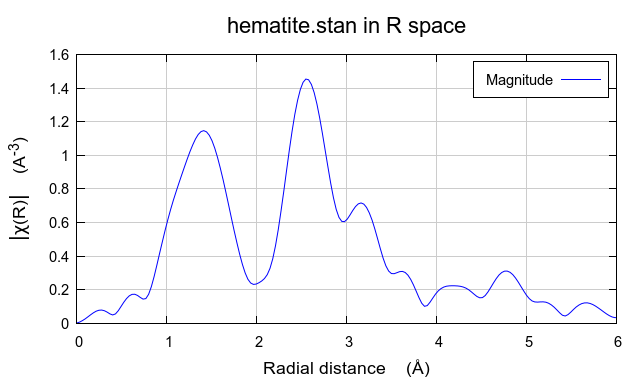
\includegraphics[width=0.5\linewidth]{hematite_chir.png}
  \end{center}

  Hematite has a known crystal structure$^\ast$ with Fe in a
  six-coordinated oxygen octahedron.  There are 3 near neighbor oxygen
  atoms at 1.95\,\AA\ and 3 others 2.12\,\AA.

  \vspace{-2ex}
  
  \begin{center}
    \begin{minipage}{0.8\linewidth}
      \begin{alertblock}{}
        Why is the first peak in $\tilde\chi(R)$ at about 1.4\,\AA\
        when the nearest neighbor is at 1.95\,\AA?
      \end{alertblock}
    \end{minipage}
  \end{center}
  \begin{bottomnote}[0.5][19]%
    $^\ast$R.L. Blake, R.E. Hessevick, T. Zoltai, L.W. Finger
    American Mineralogist 51 (1966) 123-129, \textit{Refinement of
      the hemtatite structure}
  \end{bottomnote}

\end{frame}

\begin{frame}
  \frametitle{EXAFS Equation}
  \small
  Here's the EXAFS equation:

  \exafsequation

  The oscillatory term is a function not of $2kR$, but of
  \alert{$2kR + \Phi(k)$}.
  

  \bigskip
  
  The integral that makes $\tilde\chi(R)$ is usually done over $2k$,
  i.e. $\tilde\chi(R) = \int d(2k)\, k^{kw}\cdot\chi(k)$.  This makes
  $\tilde\chi(R)$ look somewhat like a radial distribution function
  with peaks near sensible values of $R$ (half-path-length), rather
  than $2R$ (full-path-length).
\end{frame}

\begin{frame}
  \frametitle{Scattering Amplitues and Phase Shifts}
  \small
  
  Remember that the complex scattering function (for which
  $\color{Blue4}F(k)$ is the amplitude and 
  ${\color{Blue4}\Phi(k)}$ is the phase) is structured and
  Z-dependent.  Here are some representative examples for elements
  from different rows of the periodic table.
  
  \begin{columns}[T]
    \begin{column}{0.5\linewidth}
      \centering $\color{Blue4}F_\Gamma(k)$\\
      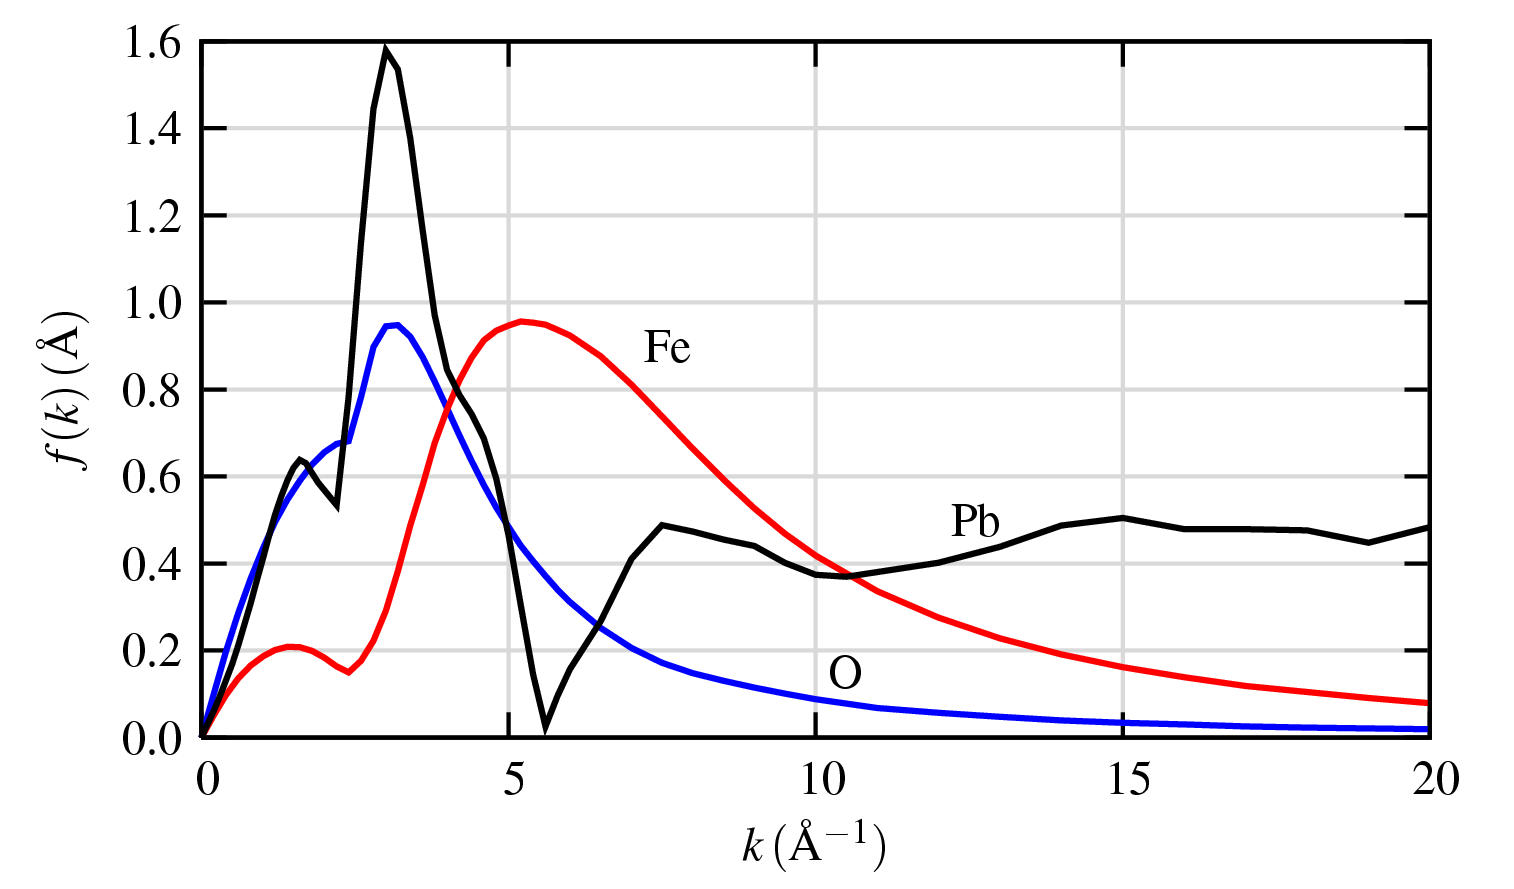
\includegraphics[width=\linewidth]{amplitudes.png}      
    \end{column}
    \begin{column}{0.5\linewidth}
      \centering ${\color{Blue4}\Phi_\Gamma(k)}$ \\
      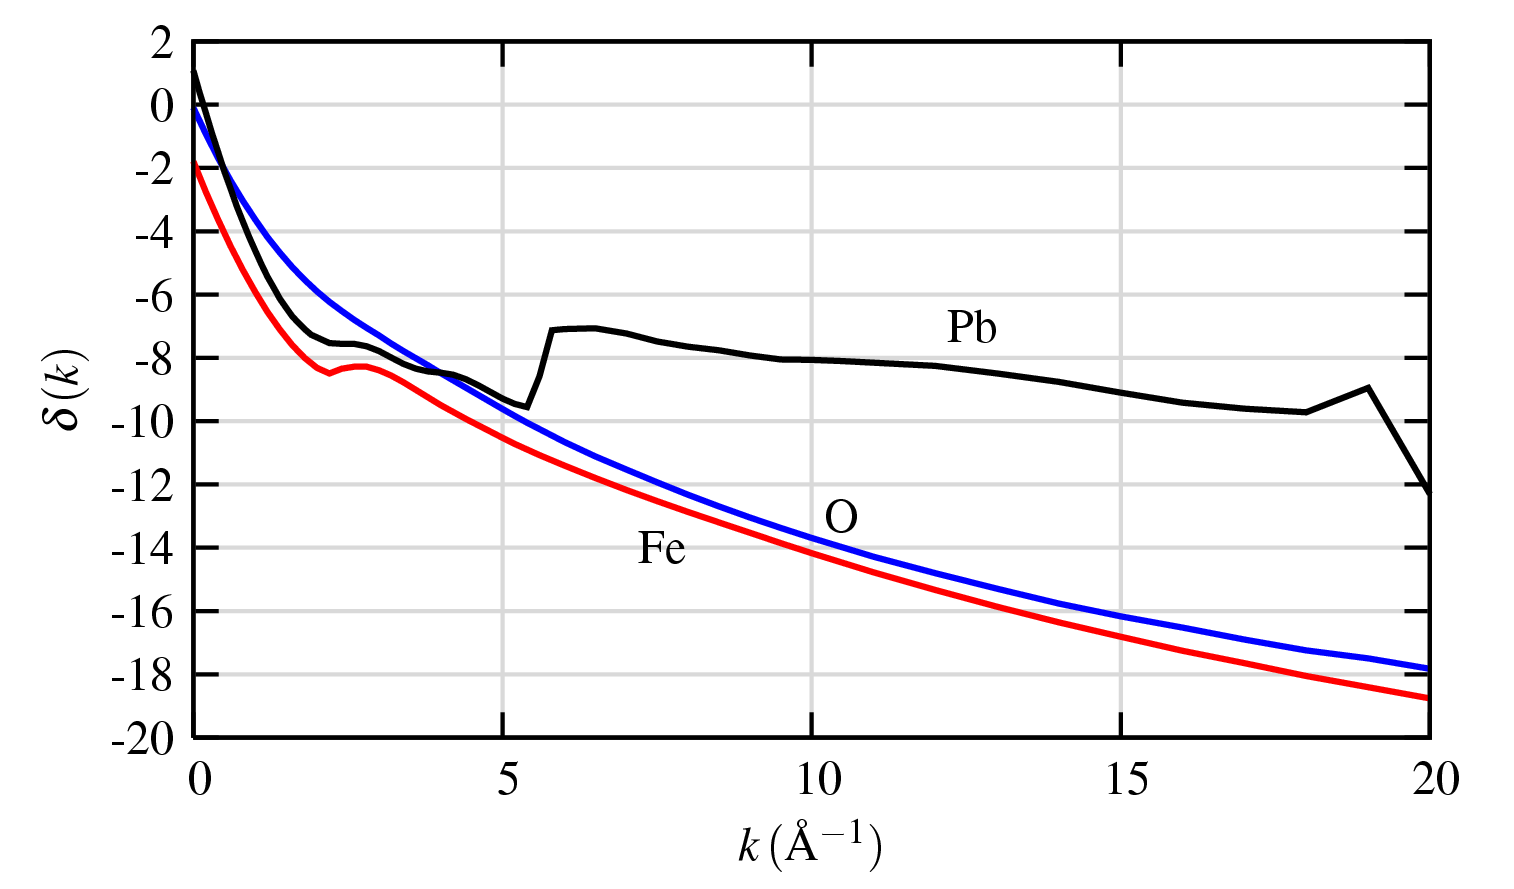
\includegraphics[width=\linewidth]{phases.png}
    \end{column}
  \end{columns}

  Very heavy elements have a discontinuity in
  ${\color{Blue4}\Phi(k)}$, like Pb at about 5.5\,\AA$^{-1}$.

  \bigskip

  Lighter scatterers, like O and Fe, have fairly smooth phase
  functions.
  
  \begin{bottomnote}[0.5][19]%
    These figures are from Matt Newville's
    \href{http://xafs.org/Tutorials?action=AttachFile&do=get&target=Newville_xas_fundamentals.pdf}{\color{LightBlue4}Fundamentals of X-ray Absorption Fine Structure}
  \end{bottomnote}
\end{frame}

\begin{frame}
  \frametitle{Examining the Phase Function}
  \small
  
  The phase functions for the lighter elements are valued near 0 at
  $k=0$\,\AA$^{-1}$ and decrease to almost 20 at $k=20$\,\AA$^{-1}$.
  To some level of approximation, these phase functions can be
  described by a line of slope -1, i.e. $\Phi(k) \approx -1\cdot k$

  \begin{center}
    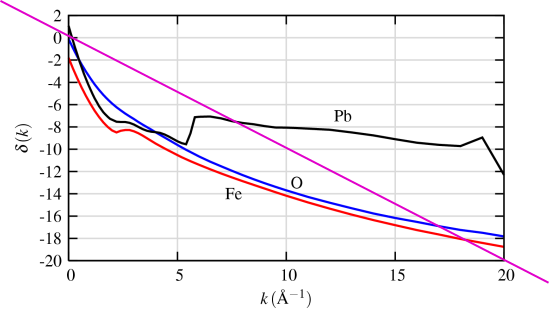
\includegraphics[width=0.5\linewidth]{slope.pdf}
  \end{center}

  Using that crude approximation, the oscillatory term of the EXAFS
  equation is $\sin(2kR - k) = \sin\big(2k\cdot(R-\frac{1}{2})\big)$.
  When the integral is done over $d(2k)$, the first peak in the
  resulting $\tilde\chi(R)$ shows up around (R-$\frac{1}{2})$\,\AA.
\end{frame}

\begin{frame}
  \frametitle{This is why the first peak is shifted inward}
  Obviously, the approximation of $\Phi(k)$ as a straight line is
  inaccurate.  The peak shift is not exactly $\frac{1}{2}$\,\AA.  And
  for heavier scatterers, the approximation is even worse.

  \bigskip

  But this explains in a hand-waving sense why the peaks are shifted
  to lower $R$ in $\tilde\chi(R)$.

  \bigskip

  This is yet another reason why $\tilde\chi(R)$ is \textbf{NOT} a
  radial distribution function.
\end{frame}
\end{document}

%%% Local Variables:
%%% mode: latex
%%% TeX-master: t
%%% TeX-parse-self: t
%%% TeX-auto-save: t
%%% TeX-auto-untabify: t
%%% TeX-PDF-mode: t
%%% End:
